\section{dg::Light Struct Reference}
\label{structdg_1_1Light}\index{dg::Light@{dg::Light}}
{\tt \#include $<$Shading.h$>$}

Collaboration diagram for dg::Light:\begin{figure}[H]
\begin{center}
\leavevmode
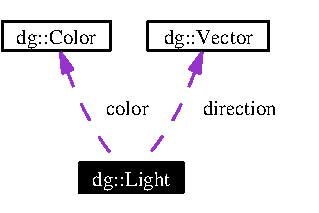
\includegraphics[width=94pt]{structdg_1_1Light__coll__graph}
\end{center}
\end{figure}
\subsection*{Public Attributes}
\begin{CompactItemize}
\item 
{\bf Vector} {\bf direction}
\item 
{\bf Real} {\bf intensity}
\item 
{\bf Color} {\bf color}
\end{CompactItemize}


\subsection{Member Data Documentation}
\index{dg::Light@{dg::Light}!color@{color}}
\index{color@{color}!dg::Light@{dg::Light}}
\subsubsection{\setlength{\rightskip}{0pt plus 5cm}{\bf Color} dg::Light::color}\label{structdg_1_1Light_m2}




Definition at line 18 of file Shading.h.\index{dg::Light@{dg::Light}!direction@{direction}}
\index{direction@{direction}!dg::Light@{dg::Light}}
\subsubsection{\setlength{\rightskip}{0pt plus 5cm}{\bf Vector} dg::Light::direction}\label{structdg_1_1Light_m0}




Definition at line 16 of file Shading.h.\index{dg::Light@{dg::Light}!intensity@{intensity}}
\index{intensity@{intensity}!dg::Light@{dg::Light}}
\subsubsection{\setlength{\rightskip}{0pt plus 5cm}{\bf Real} dg::Light::intensity}\label{structdg_1_1Light_m1}




Definition at line 17 of file Shading.h.

The documentation for this struct was generated from the following file:\begin{CompactItemize}
\item 
{\bf Shading.h}\end{CompactItemize}
